\FILENAME

Mastering a text processing system is an essential part of a
researcher's life. Not knowing how to use a text processing system can
slow down the productivity of research drastically.

\section{Installation}
\label{installation}
\index{Latex!installation}

LaTeX is available on all modern computer systems. A very good
installation for OSX is available at:

\begin{itemize}
\item
  \url{https://tug.org/mactex/}
\end{itemize}


However, if you have older versions on your systems you may have to
first completely uninstall them.

\subsection{Local Install}\label{local-install}

Installing LaTeX is trivial, and is documented on the internet very
well. However, it requires sufficient space and time as it is a large
environment. A system such as TeX Live takes in full install about 5.5
GB. In addition to LaTeX we recommend that you install jabref and use it
for bibliography management.

Thus you will have the most of them on your system.

\begin{itemize}

\item
  pdflatex: the latex program producing pdf
\item
  bibtex: to create bibliographies
\item
  jabref: GUI application to bibtex files (\url{http://www.jabref.org/})
\end{itemize}

Make sure you check that these programs are there, for example with the
Linux commands:

\begin{verbatim}
which pdflatex
which bibtex
which jabref (on OSX you may have an icon for it)
\end{verbatim}

If these commands are missing, please install them. For the newest
documentation on installation of LaTeX we recommend you look up the
installation for your specific OS.

\subsubsection{Install on Ubuntu 16.04}\label{install-on-ubuntu-16.04}
\index{Latex!installation!ubuntu}

The easiest way to install it on ubuntu is to use the terminal and type
in (make sure you have enough space):

\begin{verbatim}
sudo apt-get install texlive-full
\end{verbatim}

One of the best editors for LaTeX is emacs as you can also do
bibliography management with it and not just LaTeX. However, other
editors are available including:

\begin{itemize}

\item
  Kile, TeXworks, JLatexEditor, Gedit LaTeX Plugin, TeXMaker
\end{itemize}

Please look up how to install them if you like to use them. TeXMaker is
popular, However I find the combination of emacs and latexmk superior.
TeXmaker is installed with:

\begin{verbatim}
sudo apt-get install texmaker
\end{verbatim}

Other installations:

\begin{itemize}

\item
  kile is installed by default
\item
  \url{https://www.tug.org/texworks/} (Works on ubuntu, Windows, OSX)
\end{itemize}

\subsubsection{LaTeX for OSX}\label{latex-for-osx}
\index{Latex!installation!OSX}

\begin{itemize}

\item
  \url{https://www.latex-project.org/get/}
\end{itemize}

\subsubsection{LaTeX for Windows}\label{latex-for-windows}
\index{Latex!installation!Windows}

\begin{itemize}

\item
  \url{https://www.latex-project.org/get/}
\end{itemize}

\subsection{Online Services}\label{online-services}

\subsubsection{Sharelatex}\label{sharelatex}
\index{Latex!Sharelatex}

ShareLaTeX is an online, collaborative LaTeX editor that makes the
creation, preview, and sharing of LaTeX documents easy through a
web-based interface.  Those that like to use latex, but do not have it
installed on their computers may want to look at the following video:

Video: \url{https://youtu.be/PfhSOjuQk8Y}

Video with cc: \url{https://www.youtube.com/watch?v=8IDCGTFXoBs}

ShareLaTeX not only allows you to edit online, but allows you to share
your documents in a group of up to three. Licenses are available if you
need more than three people in a team.

\paragraph{IU Licensed ShareLaTeX}

At IU we has a license for the ShareLaTeX service available to School
of Informatics and Computing and Engineering students, faculty, and
staff only on the Bloomington campus.  

You can create a free ShareLaTeX account but the free accounts have
limitations.  Adding your account to the IU license will give you access
to advanced features, including unlimited sharing.  
It will also allow GitHub integration. THis however only works with
the commercial github.com and not the IU Enterprise GitHub at
github.iu.edu. As we require in our courses github.com you will be
able to use it.

{\em Please note that this license is only available to School of
Informatics and Computing students, faculty, and staff on the
Bloomington campus.  Students must be enrolled in one of the SoIC
degree programs on the Bloomington campus to be eligible.  Students in
other degree programs (even those taking SoIC classes) are not
eligible.}


If you want to use this service, please do and be aware of the following: 

\begin{enumerate}

\item Go to the ShareLaTeX site and register.  Please note that you
  {\bf must} use either an \verb|@indiana.edu| or \verb|@iu.edu| email
  address when you register. If you use any other email address, we
  will not be able to add you to our site license.  You are also
  required to use your IU passphrase as your ShareLaTeX password.
  Once you have registered, send an email to
  \verb|soichelp@indiana.edu| asking to have your sharelatex account 
  added to the IU license.  

\item
  In your request, you must include the following: The IU email
  address you used when you registered (which must be in either the
  \verb|@indiana.edu| or \verb|@iu.edu| domain) A statement indicating
  that you understand that the ShareLaTeX service cannot be used for
  any sensitive data

\item Note that the ShareLaTeX service is {\bf not} qualified for any
  sensitive data. This includes all data in the Critical, Restricted,
  and University-Internal categories as defined in the Data
  Classifications Page.

\end{enumerate}


\subsubsection{Overleaf}\label{overleaf}
\index{Latex!overleaf}

Overleaf.com is a collaborative latex editor. In its free version it has
a very limited disk space. However it comes with a Rich text mode that
allows you to edit the document in a preview mode. The free templates
provided do not include ACM template, put you are allowed to use the OSA
template.

Features of overleaf are documented at:
\url{https://www.overleaf.com/benefits}

\subsubsection{Paperia}\label{paperia}

We do not know where this service is located. However it offers similar
services as ShareLatex and Overleaf.

\begin{itemize}

\item
  \url{https://papeeria.com/}
\end{itemize}


\section{Basic LaTeX Elements}\label{latex}
\index{Latex!Elements}

Often researchers may be initially overwhelmed with all the features
that \LaTeX~ provides. However, it is much simpler than you initially
believe. In Chapter ?? we introduced you towards using an article
template. As a template is provided you can just look at the elements
in that article and modify or copy them while adapting the
content. Thus, it is more like filling out a form. You do not have to
learn much and you can learn as you go. We are providing in this
chapter some basic \LaTeX~ elements that will help you getting started
quickly while serving you as a reminder what how to do certain things
in \LaTeX~.



\subsection{Characters}\label{characters}
\index{Latex!\%}
\index{Latex!\$}
\index{Latex!\#}
\index{Latex!\_}

LaTeX is a command language and as such uses some special characters as
part of the language. Thus if you want to use these characters either in
your text or bibliography you need to be especially carful about. These
characters include \% \$ \# \_

Other than in hyperref links and urls you need to put a backslash in
front of them. For example to print a \% in the text you need to use:

\begin{verbatim}
\%
\end{verbatim}

Furthermore the character \verb|"| is not at all used as discussed in the next
section.

\subsection{Highlighting Text}\label{highlighting-text}
\index{Latex!Elements!highlight text}

Quotes are not written with the \verb|"| character, but are embedded in two
left single quotes and two right single quotes:



\begin{tcblisting}{colback=blue!5!white,colframe=gray!50!blue,listing side text,
  title=quote,fonttitle=\bfseries}
``This is a quote''
\end{tcblisting}



In many papers we see that the quote is misused while putting quotes
around a word. However quotes are often just used to quote a text from
another paper. Instead of using quotes authors may actually emphasize a
word. LaTeX has a special command for that using:

\begin{tcblisting}{colback=blue!5!white,colframe=gray!50!blue,listing side text,
  title=emphasize,fonttitle=\bfseries}
{\em this is emphasized}
\end{tcblisting}

To write a text as bold (which should also be avoided as bold is
typically used in section headers), you can use:

\begin{tcblisting}{colback=blue!5!white,colframe=gray!50!blue,listing side text,
  title=bold fett,fonttitle=\bfseries}
{\bf this is bold fett}
\end{tcblisting}

\subsection{Sections}\label{sections}
\index{Latex!Elements!sections}

LaTeX provides a convenient mechanism to structure a paper with sections
and subsections THis is achieved with the following commands:

\begin{verbatim}
\section{This is a Section}
\subsection{This is a Subsection}
\subsubsection{This is a Subsubsection}  
\end{verbatim}

Once you use one of these commands the next paragraph will start bellow
the section command.

In addition you have the command:

\begin{verbatim}
\paragraph{This is a paragraph.}

The line is behind the paragraph heading
\end{verbatim}

The command is special as it does not introduce a new line between the
Heading and the next line even if you include empty lines

\subsection{Empty Lines}\label{empty-lines}

Multiple empty lines will be reduced to a single empty line.

\subsection{Itemize}\label{itemize}
\index{Latex!Elements!itemiz}


Itemized lists can be written as follows:


\begin{tcblisting}{colback=blue!5!white,colframe=gray!50!blue,listing side text,
  title=itemize,fonttitle=\bfseries}
\begin{itemize}
   \item First item
   \item Second item
\end{itemize}
\end{tcblisting} 


\subsection{Enumerate}\label{enumerate}
\index{Latex!Elements!enumerate}

Enumerations can be written as:

\begin{tcblisting}{colback=blue!5!white,colframe=gray!50!blue,listing side text,
  title=enumerate,fonttitle=\bfseries}
\begin{enumerate}
   \item First item
   \item Second item
\end{enumerate}
\end{tcblisting} 

\subsection{Descriptions}\label{descriptions}
\index{Latex!Elements!description}

Description lists can be written as:

\begin{tcblisting}{colback=blue!5!white,colframe=gray!50!blue,listing side text,
  title=enumerate,fonttitle=\bfseries}
\begin{description}
   \item[Cloud:] My definition of a Cloud is over more than one line
     so we show the indentation.
   \item[Big Data:] My definition of Big Data is also a long description.
\end{description}
\end{tcblisting} 




\subsection{Images}\label{images}
\index{Latex!Elements!images}

Figures are extremely easy to handle by including them from source. We
never worry about the placement as LaTeX does typically a very
good job of doing this.:

\begin{verbatim}
In Figure \ref{F:flow} we show a black and white graph about ... .

\begin{figure}[htb]
  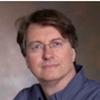
\includegraphics[width=1.0\columnwidth]{images/gregor.png}
  \caption{A demonstration in the scalability of PDF images.}
  \label{F:flow}
\end{figure}
\end{verbatim}

Which results in the following:
\begin{quote}
In Figure \ref{F:flow} we show a black and white graph about ... .

\begin{figure}[htb]
  \includegraphics[width=1.0\columnwidth]{images/i523-overview.pdf}
  \caption{A demonstration in the scalability of PDF images.}
  \label{F:flow}
\end{figure}
\end{quote}

Note that las17graph must be a label of a valid bibtex entry. This is
needed if you have copied the image from elsewhere to avoid plagiarism.
However, if you came up with the graph yourself than you do not need a
citation.

We recommend that you place in your paper drafts all images at the which
can be done with the endfloat package

This can be enabled if you include the following lines before begin
document command:

\begin{verbatim}
\usepackage{endfloat}
\renewcommand{\efloatseparator}{\mbox{}} 

\begin{document}
\end{verbatim}

\subsection{Tables}\label{tables}
\index{Latex!Elements!tables}

Latex tables are very similar to csv table. Thus you could with
appropriate manipulation create tables from csv tables and use tools
such as spreadsheet editors to manage your table. There are even
packages that allow you to import the contents of csv tables directly
into \LaTeX.

In many cases you simply can start with an online table generator such as

\URL{https://www.tablesgenerator.com/}

For some tables you may want to rescale the width with

\begin{verbatim}
\resizebox{\textwidth}{!}{%
   ... PUT YOUR TABLE HERE ....
}
\end{verbatim}

In other cases you may want to rotate the table which you can easily
google for. In all cases use as figures, tables need to be in the
\verb|table| float environment. In contrast to figures captions are on
the top. All tables must be referred to by \verb|ref|. For more
information in directly including csv tables see 

\URL{http://mirror.utexas.edu/ctan/macros/latex/contrib/csvsimple/csvsimple.pdf}

However the format is very easy and can in most cases directly be
included in latex as shown in Table \ref{T:elements}.

\begin{verbatim}
\begin{table}[htb]
\caption{Table with elements}\label{T:elements}
\bigskip
\begin{center}
\begin{tabular}{ c c c }
 column1  & column2  & column3 \\
\hline
\hline
 element1 & element2 & element3 \\ 
 element4 & element5 & element6 \\  
 element7 & element8 & element9 \\
\hline
\end{tabular}
\end{center}
\end{table}
\end{verbatim}

\begin{table}[htb]
\caption{Table with elements}\label{T:elements}
\bigskip
\begin{center}
\begin{tabular}{ c c c }
 column1  & column2  & column3 \\
\hline
\hline
 element1 & element2 & element3 \\ 
 element4 & element5 & element6 \\  
 element7 & element8 & element9 \\
\hline
\end{tabular}
\end{center}
\end{table}

\subsection{Labels}\label{labels}
\index{Latex!Elements!labels}

As we saw already for figures and tables it is recommended to use the
label and ref commands to refer to figure or table numbers. This applies
also to sections. Thus I can place a label after a section:

\begin{verbatim}
\section{Introduction}\label{S:introduction}
\end{verbatim}

and write elsewhere in the paper:

\begin{verbatim}
As we showcased in Section \ref{S:introduction}
\end{verbatim}

Furthermore to conveniently distinguish sections tables and figures, we
use the prefix S T F followed by a colon for the label. This helps
organizing your paper in case you have many labels.

\subsection{Mathematics}\label{math}
\index{Latex!Elements!mathematics}

One of the strength of LaTeX thi the ability to write easily
sophisticated mathematical expressions on paper with high quality. A
good online resource is provided by the following online resource from
which we have copied some examples:

\begin{itemize}

\item
  \url{https://en.wikibooks.org/wiki/LaTeX/Mathematics}
\end{itemize}

To activate them use 

\begin{verbatim}
\usepackage{amsmath}
\end{verbatim}

at the beginning of the document after the document class

Exponents are using the \^{} character:

\begin{tcblisting}{colback=blue!5!white,colframe=gray!50!blue,listing side text,
  title=exponents,fonttitle=\bfseries}
$(a+b)^2 = a^2 + 2ab + b^{c+2}$
\end{tcblisting} 

Greek letters are referred to by their name proceeded by the slash:

\begin{tcblisting}{colback=blue!5!white,colframe=gray!50!blue,listing side text,
  title=greek,fonttitle=\bfseries}
$ \alpha \beta \gamma \Gamma \pi \Pi \phi $
\end{tcblisting}


Limits can be written as follows:

\begin{tcblisting}{colback=blue!5!white,colframe=gray!50!blue,listing side text,  title=limits,fonttitle=\bfseries}
$ \lim_{x \to \infty} \exp(-x) = 0 $
\end{tcblisting}

Fractions are indicated by the frac command, and binomials by binom:

\begin{tcblisting}{colback=blue!5!white,colframe=gray!50!blue,listing side text,  title=fraction,fonttitle=\bfseries}
$ \frac{n!}{k!(n-k)!} = \binom{n}{k} $   
\end{tcblisting}

Matrices can be created as follows:

\begin{tcblisting}{colback=blue!5!white,colframe=gray!50!blue,listing side text,  title=matrix,fonttitle=\bfseries}
$ A_{m,n} = 
\begin{pmatrix}
  a_{1,1} & a_{1,2} & \cdots & a_{1,n} \\
  a_{2,1} & a_{2,2} & \cdots & a_{2,n} \\
  \vdots  & \vdots  & \ddots & \vdots  \\
  a_{m,1} & a_{m,2} & \cdots & a_{m,n} 
\end{pmatrix} $
\end{tcblisting}



\section{Advanced topics}

\subsection{ACM and IEEE Proceedings Format}\label{acm-proceedings-format}
\index{Latex!proceedings!acm}
\index{Latex!proceedings!ieee}

\begin{figure}[!h]
  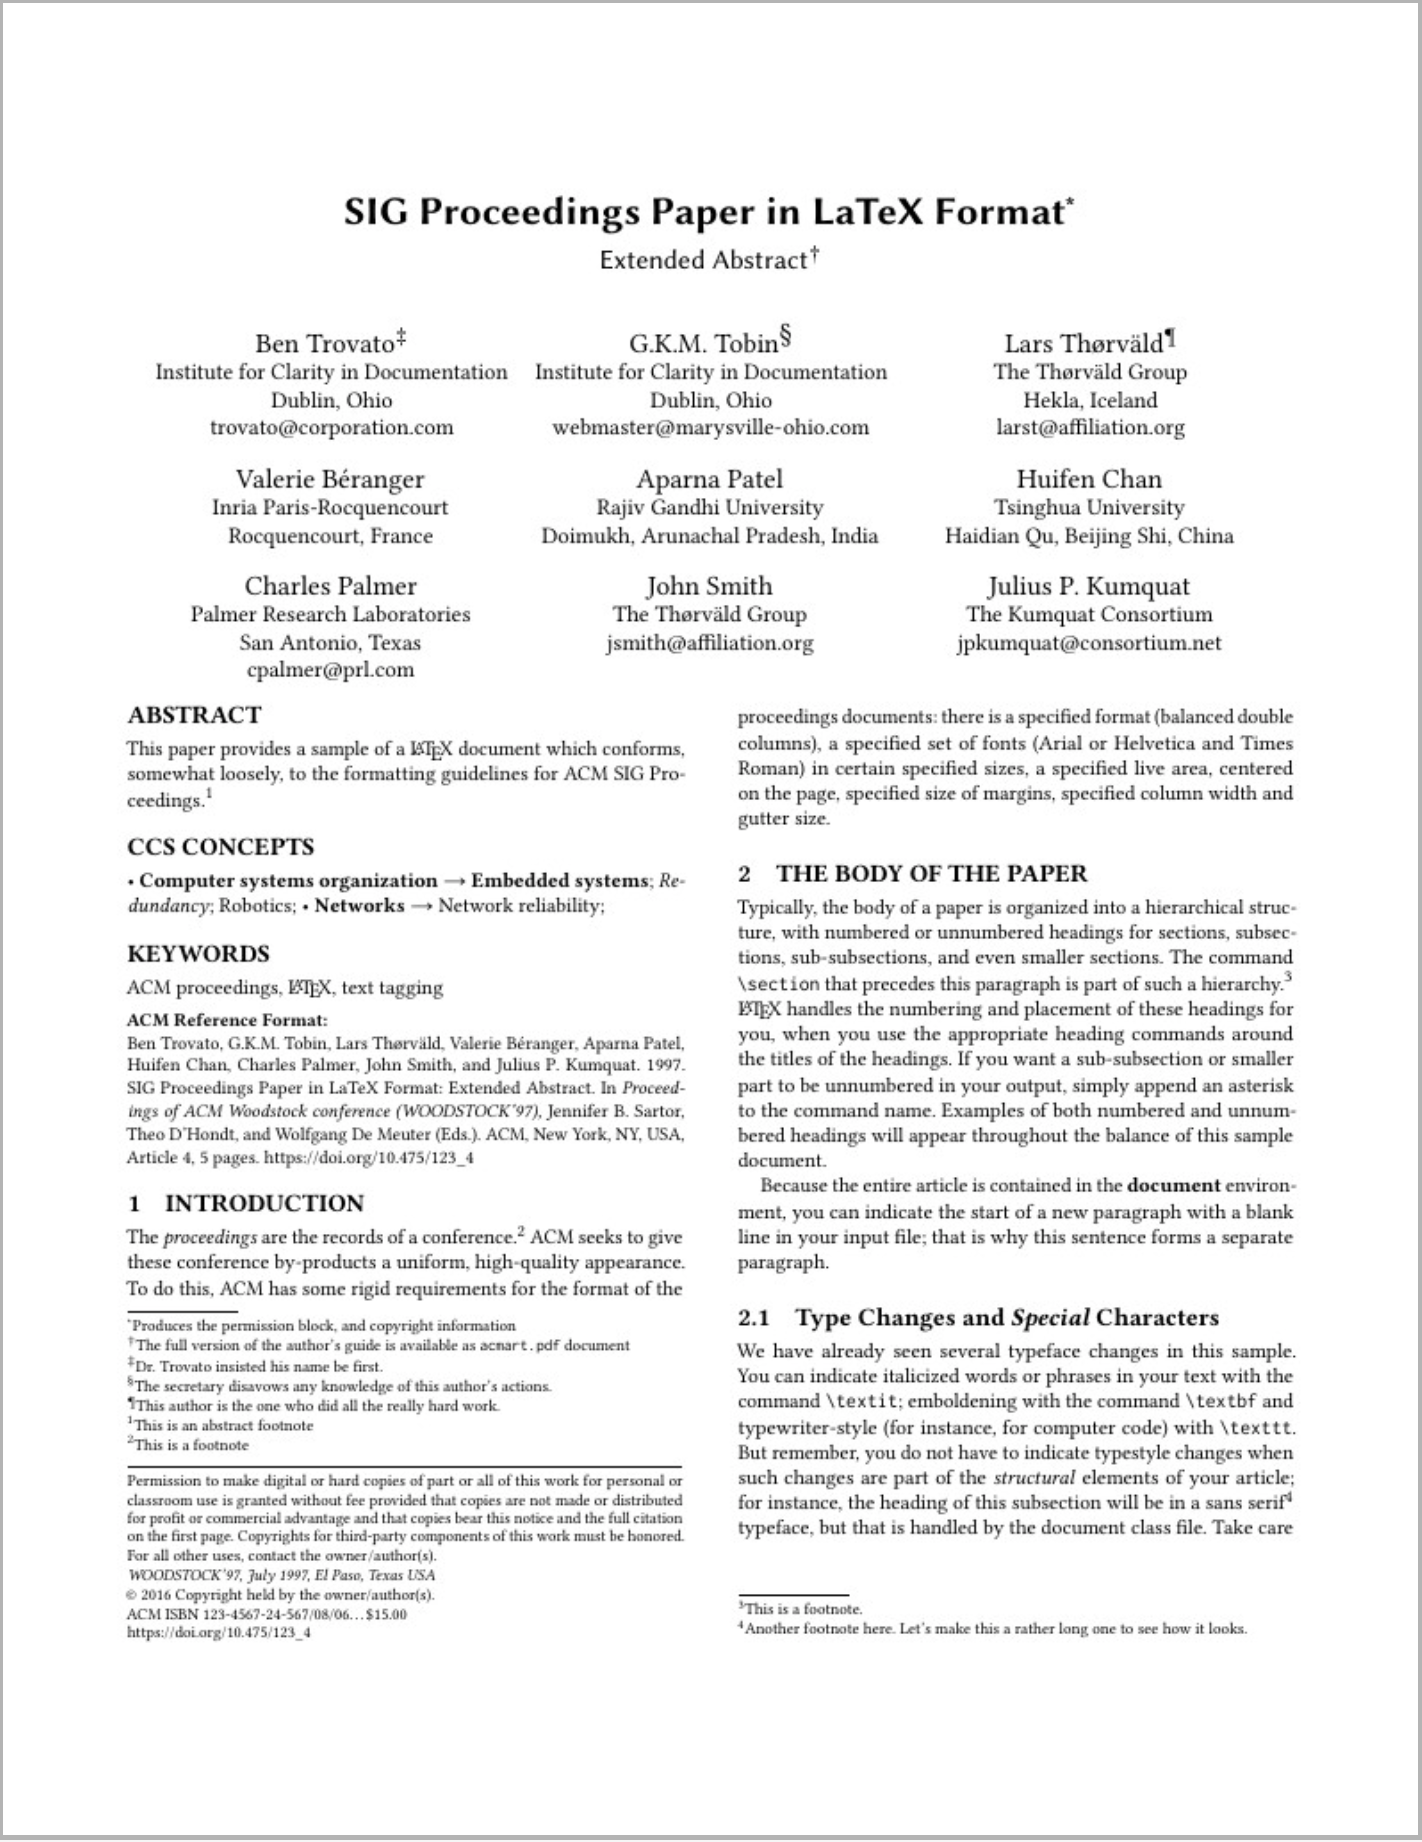
\includegraphics[width=6cm]{images/doc/acm.png}
  \hfill
  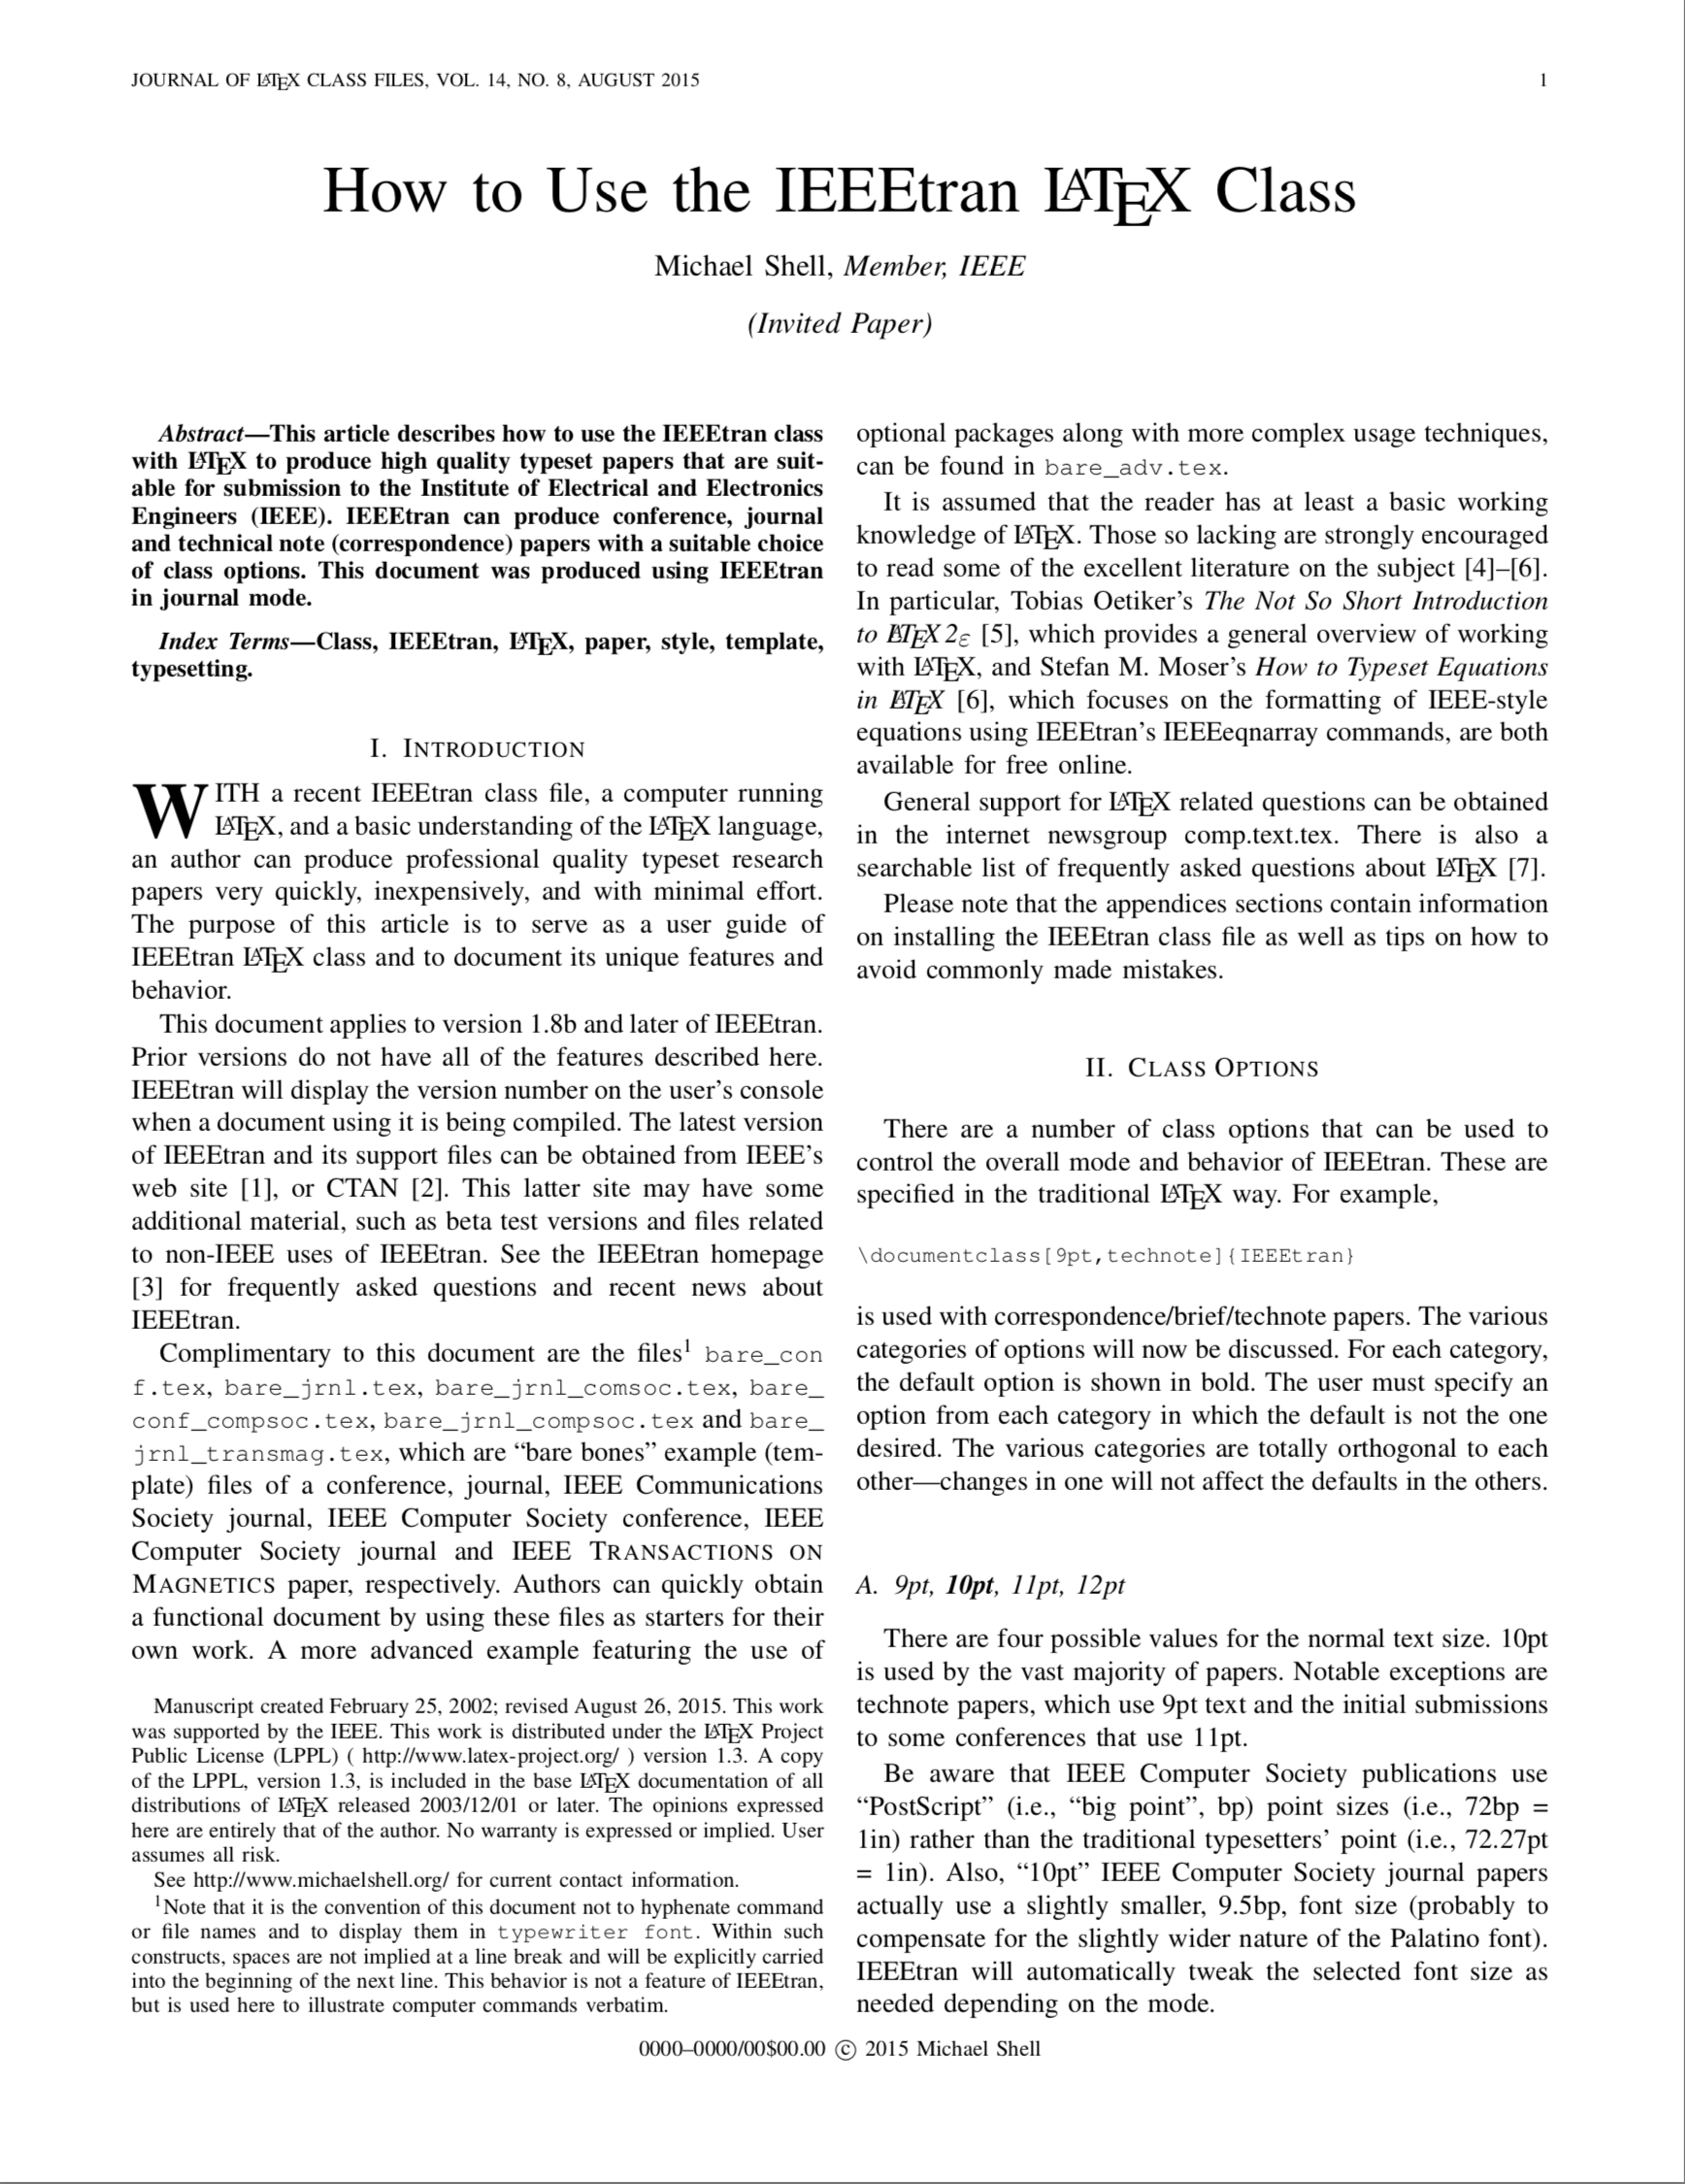
\includegraphics[width=6cm]{images/doc/ieee.png}
\caption{The look of the ACM and IEEE format templates}
\end{figure}

\begin{itemize}

\item
  \url{http://www.acm.org/publications/proceedings-template}
\item
  \url{https://www.ieee.org/conferences_events/conferences/publishing/templates.html}
\end{itemize}

\subsection{Generating and Managing Images}\label{generating-images}

To produce high quality images the programs PowerPoint and omnigraffle
on OSX are recommended. When using powerpoint please keep the image
ratio to 4x3 as they produce nice size graphics which you also can use
in your presentations. When using other rations they may not fit in
presentations and thus you may increase unnecessarily your work. We do
not recommend vizio as it is not universally available and produces
images that in case you have to present them in a slide presentation
does not easily reformat if you do not use 4x3 aspect ratio.

Naturally, graphics should be provided in SVG or PDF format so they can
scale well when we look at the final PDF. Including PNG, gif, or jpeg
files often do not result in the necessary resolution or the files
become real big. For this reason we for example can also not recommend
tools such as tablaeu as they do not provide proper exports to high
quality publication formats. For interactive display such tool may be
good, but for publications it produces inferior formatted images.

We recommend that all images be stored into a folder called images in
the same directory where your \LaTeX~ main document resides.



\subsection{Colored Boxes}

The package \verb|tcolorbox| provides sophisticated support to include
color boxes. Together with the new environment we can create nice add
ons to for example include notes.

\URL{http://osl.ugr.es/CTAN/macros/latex/contrib/tcolorbox/tcolorbox.pdf}

We have provided in this document notes as follows


\begin{tcblisting}{colback=blue!5!white,colframe=gray!50!blue,listing side text,  title=Note,fonttitle=\bfseries}
\begin{NOTE}
This is a note
\end{NOTE}
\end{tcblisting}

\begin{tcblisting}{colback=blue!5!white,colframe=gray!50!blue,listing side text,  title=Warning,fonttitle=\bfseries}
\begin{WARNING}
This is a note
\end{WARNING}
\end{tcblisting}


\subsection{Slides}\label{slides}
\index{Latex!slides}

Slides are best produced with the seminar package:

\begin{verbatim}
\documentclass{seminar}

\begin{slide}

    Hello World on slide 1

\end{slide}

The text between slides is ignored

\begin{slide}

    Hello World on slide 2

\end{slide}
\end{verbatim}

However, in case you need to have a slide presentation we recommend you
use ppt. Just paste and copy content from your PDF or your LaTeX source
file into the ppt.



\subsection{LaTeX vs. X}\label{latex-vs.-x}

We will refrain from providing a detailed analysis on why we use LaTeX
in many cases versus other technologies. In general, we find that LaTeX:

\begin{itemize}

\item
  is incredibly stable
\item
  produces high-quality output
\item
  is platform independent
\item
  has lots of templates
\item
  has been around for many years so it works well
\item
  removes you from the pain of figure placements
\item
  focusses you on content rather tan the appearance of the paper
\item
  integrates well with code repositories such as git to write
  collaborative papers.
\item
  has superior bibliography integration
\item
  has a rich set of tools that make using LaTeX easier
\item
  authors do not play with layouts much so papers in a format are
  uniform
\end{itemize}

In case you need a graphical view to edit LaTeX or LateX exportable
files you also find AucTeX and Lyx.

\subsubsection{Word}\label{word}

Word is arguably available to many, but if you work on Linux you may be
out of luck. Also Word often focusses not on structure of the text but
on its appearance. Many students abuse Word and the documents in Word
become a pain to edit with multiple users. Recently Microsoft has
offered online services to collaborate on writing documents in groups
which work well. Integration with bibliography managers such as endnote
or Mendeley is possible.

However, we ran into issues whenever we use word:

\begin{itemize}

\item
  Word tends sometimes to crash for unknown reasons and we lost a lot of
  work
\item
  Word has some issues with the bibliography managers and tends to crash
  sometimes for unknown reasons.
\item
  Word is slow with integration to large bibliographies.
\item
  Figure placement in Word in some formats is a disaster and you will
  spend many hours to correct things just to find out that if you make
  small changes you have to spend additional many hours to get used to
  the new placement. We have not yet experienced a word version where we
  have not lost images. Maybe that has changed, so let us know
\end{itemize}

However, we highly recommend the collaborative editing features of Word
that work on a paragraph and not letter level. Thus saving is essential
so you do not block other people from editing the paragraph.

\subsubsection{Google Docs}\label{google-docs}

Unfortunately, many useful features got lost in the new google docs.
However, it is great to collaborate quickly online, share thoughts and
even write your latex documents together if you like (just copy your
work in a file offline and use latex to compile it ;-) )

The biggest issue we have with Google Docs is that it does not allow the
support of 2 column formats, that the bibliography integration is
non-existent and that paste and copy from web pages and images
encourages unintended plagiarism when collecting information without
annotations (LaTeX and Word are prone to this too, but we found from
experience that it tends to happen more with Google docs users.

\subsubsection{A Place for Each}\label{a-place-for-each}

When looking at the tools we find a place for each:

\begin{description}
\item[Google docs:]
Short meeting notes, small documents, quick online collaborations to
develop documents collaboratively at the same time.
\item[Word:]
Available to many, supports 2 column format, supports paragraph based
collaborative editing, Integrates with bibliography managers.
\item[LaTeX:]
Reduces failures, great offline editing, superior bibliography
management, superior image placement, runs everywhere. Great
collaborative editing with sharelatex, allows easy generation of
proceedings written by hundreds of people with shared index.
\item[The best choice for your class:]
LaTeX
\end{description}

\section{Editing}\label{editing}

\subsection{Emacs}\label{emacs}

The text editor emacs provides a great basis for editing TeX and LaTeX
documents. Both modes are supported. In addition there exists a color
highlight module enabling the color display of LaTeX and TeX commands.
On OSX aquaemacs and carbon emacs have build in support for LaTeX. Spell
checking is done with flyspell in emacs.

\subsubsection{Aquamacs}

Aquamacs is an editor based on GNU Emacs that runs on OSX and
integrates with the OSX desktop. This is for many the preferred editor
on OSX for \LaTeX.

\url{http://aquamacs.org}

\begin{figure}[!htb]
  \centering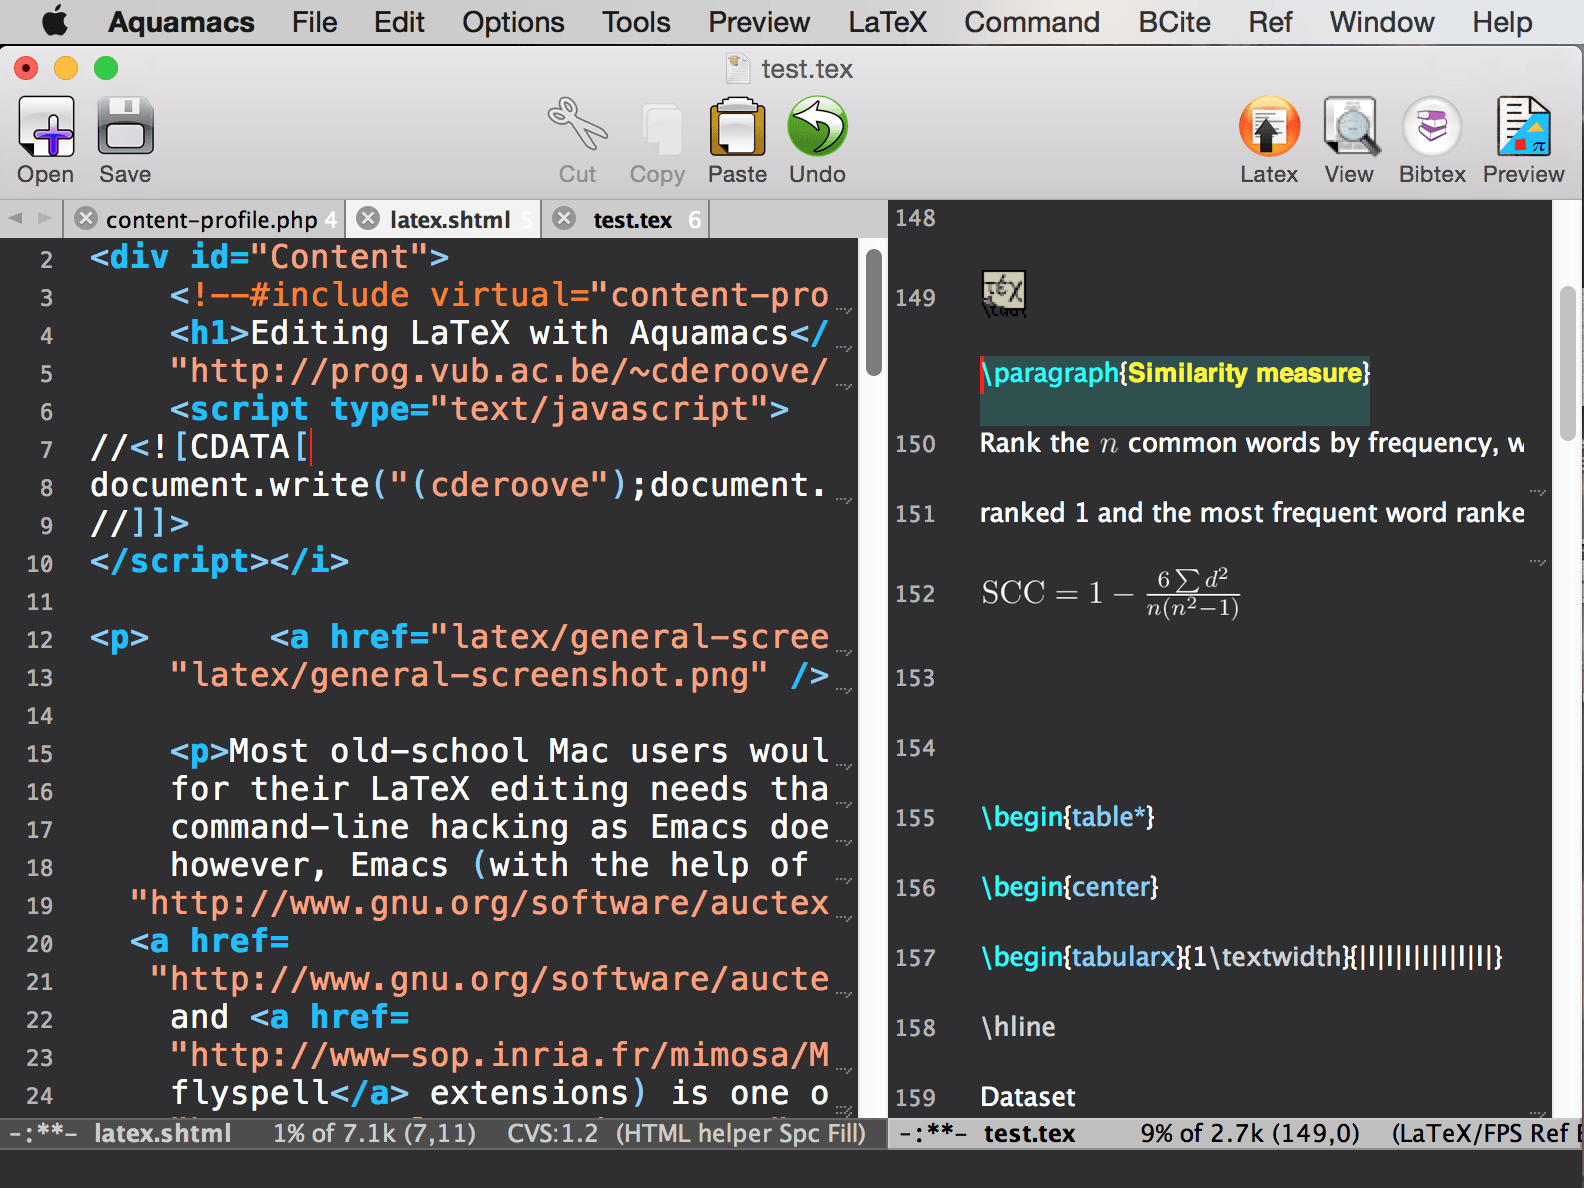
\includegraphics[width=8cm]{images/aquamacs.png}
  \caption{Aquamacs}
  \label{F:aquamacs}
\end{figure}


\subsection{Vi/Vim}\label{vivim}

Another popular editor is vi or vim. It is less feature rich but many
programmers ar using it. As it can edit ASCII text you can edit LaTeX.
With the LaTeX add-ons to vim, vim becomes similar powerful while
offering help and syntax highlighting for LaTeX as emacs does. (The
authors still prefer emacs)

\subsection{TeXshop}\label{texshop}

Other editors such as TeXshop are available which provide a more
integrated experience. However, we find them at times to stringent and
prefer editors such as emacs.

\subsection{LyX}\label{lyx}

We have made very good experiences with Lyx. You must assure that the
team you work with uses it consistently and that you all use the same
version.

\begin{figure}[!htb]
  \centering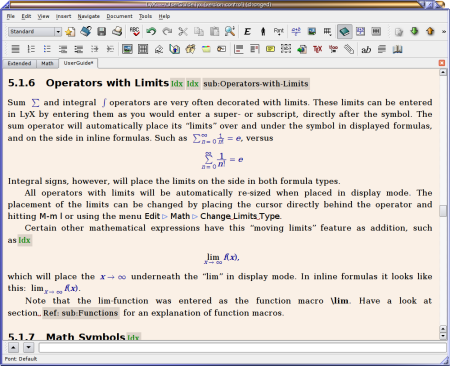
\includegraphics[width=8cm]{images/lyx.png}
  \caption{Lyx}
  \label{F:lyx}
\end{figure}

Using the ACM templates is documented here:

\begin{itemize}

\item
  \url{https://wiki.lyx.org/Examples/AcmSiggraph}
\end{itemize}

On OSX it is important that you have a new version of LaTeX and Lyx
installed. As it takes up quite some space, you ma want to delete older
versions. The new version of LyX comes with the acmsigplan template
included. However on OSX and other platforms the .cls file is not
included by default. However the above link clearly documents how to fix
this.

\subsection{WYSIWYG locally}\label{wysiwyg-locally}

We have found that editors such as Lyx and Auctex provide very good
WYSIWYG alike features. However, we found an even easier way while using
skim, a pdf previewer, in conjunction with emacs and latexmk. This can
be achieved while using the following command assuming your latex file
is called `report.tex`:

\begin{verbatim}
latexmk -pvc -view=pdf report
\end{verbatim}

This command will update your pdf previewer (make sure to use skim)
whenever you edit the file report.tex and save it. It will maintain via
skim the current position, thus you have a real great way of editing in
one window, while seeing the results in the other.

Skim can be found at: \url{http://skim-app.sourceforge.net/}

\subsection{Markdown and \LaTeX}
\index{Latex!markdown}

It may come as a surprise to many that one can actually write simple
LaTeX documents also in markdown Syntax or mix section written in
markdown while others are written in LaTeX. To do so all you ahve to
do is place the markdown text in a separate file. Let us call the file 
\verb|content.md| which has the following lines included in it:

\begin{verbatim}
# Section

* item a
* item b
\end{verbatim}

Obviously, we would have to convert this to LaTeX. Luckily there is a
very useful program called {\em pandoc} that does this for you. YOu
could make the translation in the shell, but you could also make the
translation locally on your computer while allowing \LaTeX~ to start up
external programs. This is achieved with the {\em write18} command and
allowing LaTeX explicitly to call external programs. Please inspect
the following latex file that includes a template on how to do
this. We assume the file is called markdown.tex for our example.

\begin{verbatim}
\documentclass{article}

\include{graphicx}
\newcommand{\tightlist}{}

\begin{document}
\immediate\write18{pandoc content.md -o content.tex}

\input{content}

\end{document}
\end{verbatim}

Now to generate the PDF we simply have to call the following command
that include the {\em -shell-escape} flag to allow the execution of
write18 embedded commands:

\begin{verbatim}
pdflatex -shell-escape markdown-test
\end{verbatim}

The output will be {\em markdown.pdf} with the content from the
markdown file translated. Doing this naturally allows you to write
large portions in markdown and automatically include them in your
LaTeX document. Hence, you can use editors such as Macdown to initially
work in semi WYSIWYG mode and do fairly straight forward
edition. Naturally the same can be done in RST. Naturally the most
elementary features are supported. For more sophisticated features,
please use LaTeX directly.


\subsection{Including RST into LaTeX}

content.rst:

\begin{verbatim}
Section
-------

* item a
* item b
\end{verbatim}

sample.tex:

\begin{verbatim}
\documentclass{article}

\include{graphicx}
\newcommand{\tightlist}{}

\begin{document}
\immediate\write18{pandoc content.rst -o content.tex}

\input{content}

\end{document}
\end{verbatim}


\subsection{pyCharm}

TODO: comment on how we can use pycharm for editing and what the
limitations are.

\subsection{MSWord}

it is possible to use Word.

be careful with 

\section{The LaTeX Cycle}\label{the-latex-cycle}
\index{Latex!cycle}

To create a PDF file from latex yo need to generate it following a
simple development and improvement cycle.

First, Create/edit ASCII source file with \texttt{file.tex} file:

\begin{verbatim}
emacs file.tex
\end{verbatim}

Create/edit bibliography file:

\begin{verbatim}
jabref refs.bib
\end{verbatim}

Create the PDF:

\begin{verbatim}
pdflatex file
bibtex file
pdflatex file
pdflatex file
\end{verbatim}

View the PDF:

\begin{verbatim}
open file
\end{verbatim}

It not only showcases you an example file in ACM 2 column format, but
also integrates with a bibliography. Furthermore, it provides a sample
Makefile that you can use to generate view and recompile, or even
autogenerate. A compilation would look like:

\begin{verbatim}
make
make view
\end{verbatim}

If however you want to do things on change in the tex file you can do
this automatically simply with:

\begin{verbatim}
make watch
\end{verbatim}

for make watch its best to use skim as pdf previewer


\section{Tips}\label{tips}

Including figures over two columns:

\begin{itemize}
\item
  \url{http://tex.stackexchange.com/questions/30985/displaying-a-wide-figure-in-a-two-column-document}
\item
  positioning figures with textwidth and columnwidth
  \url{https://www.sharelatex.com/learn/Positioning_images_and_tables}
\item
  An organization as the author. Assume the author is National Institute
  of Health and want to have the author show up, please do:

\begin{verbatim}
key= {National Institute of Health},
author= {{National Institute of Health}},
\end{verbatim}

  Please note the \{\{ \}\}
\item
  words containing `fi' or `ffi' showing blank places like below after
  recompiling it: find as nd efficiency as e ciency

  You copied from word or PDF ff which is actually not an ff, but a
  condensed character, change it to ff and ffi, you may find other such
  examples such as any non ASCII character. A degree is for example
  another common issue in data science.
\item
  do not use \textbar{} \& and other latex characters in bibtex
  references, instead use , and the word and
\item
  If you need to use \_ it is \_ but if you use urls leave them as is
\item
  We do recommend that you use sharelatex and jabref for writing papers.
  This is the easiest solution and beats in many cases MSWord as you can
  focus on writing and not on formatting.
\end{itemize}

\subsection{Colorful Output}

Instead of using pdflatex, you can also install \verb|pydflatex| that
provides a convenient wrapper and colorizes the output while
eliminating a lot of warnings that you may initially not want to deal
with. To install it please use:

\begin{verbatim}
pip install blessings
pip install -e "git+https://github.com/olivierverdier/pydflatex#egg=pydflatex"
\end{verbatim}

You can see the manual page with 

\begin{verbatim}
pydflatex --help

usage: usage: pydflatex [options] texfile1

Compile a tex file with pdflatex and make the auxiliary files invisible. Note
that the '.tex' extension may be omitted

positional arguments:
  tex path            path to tex file

optional arguments:
  -h, --help          show this help message and exit
  -o, --open          view the pdf file(s) in a pdf viewer.
  -k, --continue      continue on error
  -w, --with-warning  do not suppress common warnings
  -v, --verbose       Verbose output for debugging
  -p, --plain         No coloured output
  -x, --xetex         Use XeLaTeX engine
  -l, --log-parsing   Only parse log
  -t, --typesetting   Only typeset
\end{verbatim}

\subsection{latex2html}

\LaTeX~ can be exported to html with the the tool
\verb|latex2html|. It is available 

for Linux and OSX. More information can be found at

\URL{http://mirrors.ctan.org/support/latex2html/manual.pdf}

\URL{www.latex2html.org}

\begin{WARNING}
At this time the inastallation via brew install of latex2html is
broken. Instead one needs to conduct the insalation from source.

\begin{verbatim}
brew install latex2html
\end{verbatim}
\end{WARNING} 

The instalation from source can be conducted as follows

\begin{verbatim}
brew install libpng
wget https://github.com/latex2html/latex2html/archive/master.zip
uzip master.zip 
cd latex2html-master/
configure
make
make check
sudo make install
\end{verbatim}

\subsection{References}
\index{Latex!other documentation}

\begin{description}


\item[Latex Sheet:]    \url{https://wch.github.io/latexsheet/latexsheet.pdf}

\item[Latex Short:]    \url{http://tug.ctan.org/info/lshort/english/lshort.pdf}

\item[Wikibook:]       \url{https://en.wikibooks.org/wiki/LaTeX}
\item[Wikibook (PDF)]: \url{https://upload.wikimedia.org/wikipedia/commons/2/2d/LaTeX.pdf}

\item [Links to books:] \url{https://latexforhumans.wordpress.com/2008/10/11/the-best-guides-to-latex/}
\item [Links to books:] \url{https://www.latex-project.org/help/books/}
\item [LaTeX2e:]
  The
  \href{http://texdoc.net/texmf-dist/doc/latex/latex2e-help-texinfo/latex2e.pdf}{LaTeX
  Reference Manual} provides a good introduction to Latex.

\end{description}


\begin{itemize}

\item
  LaTeX Users and Reference Guide, by Leslie Lamport
  \url{https://www.amazon.com/LaTeX-Document-Preparation-System-2nd/dp/0201529831/ref=sr_1_2?s=books\&ie=UTF8\&qid=1507114870\&sr=1-2\&keywords=lamport}
\item
  LaTeX an Introduction, by Helmut Kopka
  \url{https://www.amazon.com/Guide-LaTeX-4th-Helmut-Kopka/dp/0321173856/ref=pd_lpo_sbs_14_t_0?_encoding=UTF8\&psc=1\&refRID=2BB4APDFEX34A4JM65ZB}
\item
  The LaTeX Companion, by Frank Mittelbach
  \url{https://www.amazon.com/LaTeX-Companion-Techniques-Computer-Typesetting/dp/0201362996}
\end{itemize}

